\documentclass[fullscreen=true, bookmarks=true, hyperref={pdfencoding=unicode}]{beamer}
\usepackage[utf8]{inputenc}                                % Кодировка
\usepackage[english,russian]{babel}                        % Переносы
\usepackage{xcolor}                                        % Работа с цветом
\usepackage{amsmath,amssymb,amsfonts}                      % Символы АМО
\usepackage{graphicx}                                      % Графика
\usepackage[labelsep=period]{caption}                      % Разделитель в подписях к рисункам и таблицам
\usepackage{hhline}                                        % Для верстки линий в таблицах
\usepackage{tikz}                                          % Для простых рисунков в документе
\usepackage{fancybox}                                      % Пакет для отрисовки рамок
\usepackage{verbatim}                                      % Для вставки кода в презентацию
\usepackage{animate}                                       % Для вставки видео в презентацию
\usepackage{xmpmulti}                                      % Для вставки gif в презентацию
\usepackage{multirow}

\usetikzlibrary{arrows,snakes,backgrounds}                 % Для отрисовки стрелок

\graphicspath{{images/}}                                   % Путь до рисунков
\setbeamertemplate{caption}[numbered]                      % Включение нумерации рисунков

\definecolor{links}{HTML}{2A1B81}                          % blue for url links
\hypersetup{colorlinks,linkcolor=,urlcolor=links}          % nothing for others

\usetheme{boxes}
\usecolortheme{crane}

\newtheorem*{question}{Вопрос}

\title{Лекция 1. Свёрточные нейронные сети}
\author{Александр Юрьевич Авдюшенко}
\institute{МКН СПбГУ}
\date{17 февраля 2022}
\titlegraphic{
\includegraphics[keepaspectratio,width=0.5\textwidth]{logo_fmkn.png}}

\begin{document}
%\unitlength=2mm

% выводим заглавие
\begin{frame}
\transdissolve[duration=0.2]
\titlepage
\end{frame}

\begin{frame}
  \frametitle{План второй части машинного обучения}
  \framesubtitle{Критерии оценок}
  Всё уже \href{https://github.com/spbu-math-cs/ml-course/blob/main/2022-spring-part-2/plan_and_hws.md}{в гитхабе}.
\end{frame}


{ % all template changes are local to this group.
    \setbeamertemplate{navigation symbols}{}
    \begin{frame}<article:0>[plain]
        \begin{tikzpicture}[remember picture,overlay]
            \node[at=(current page.center)] {
                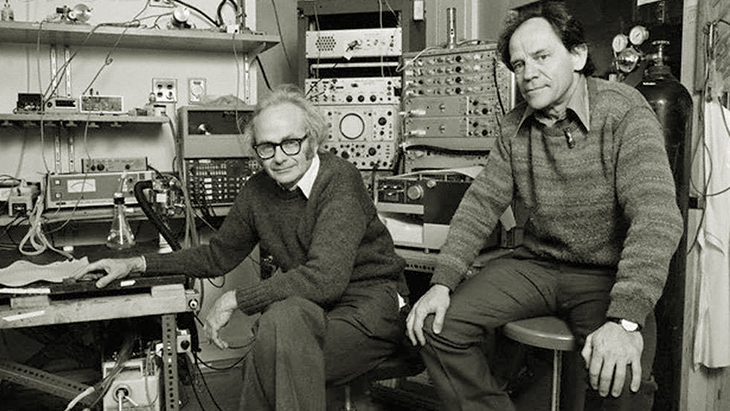
\includegraphics[keepaspectratio,
                                 width=\paperwidth,
                                 height=\paperheight]{img_EP_hubel-weisel-toys2.jpg}
            };
        \end{tikzpicture}
     \end{frame}
}


\begin{frame}
  \frametitle{Hubel \& Wiesel (1959)}
  \framesubtitle{История}
  The Nobel Prize in Physiology or Medicine, 1981
\end{frame}


{ % all template changes are local to this group.
    \setbeamertemplate{navigation symbols}{}
    \begin{frame}<article:0>[plain]
        \begin{tikzpicture}[remember picture,overlay]
            \node[at=(current page.center)] {
                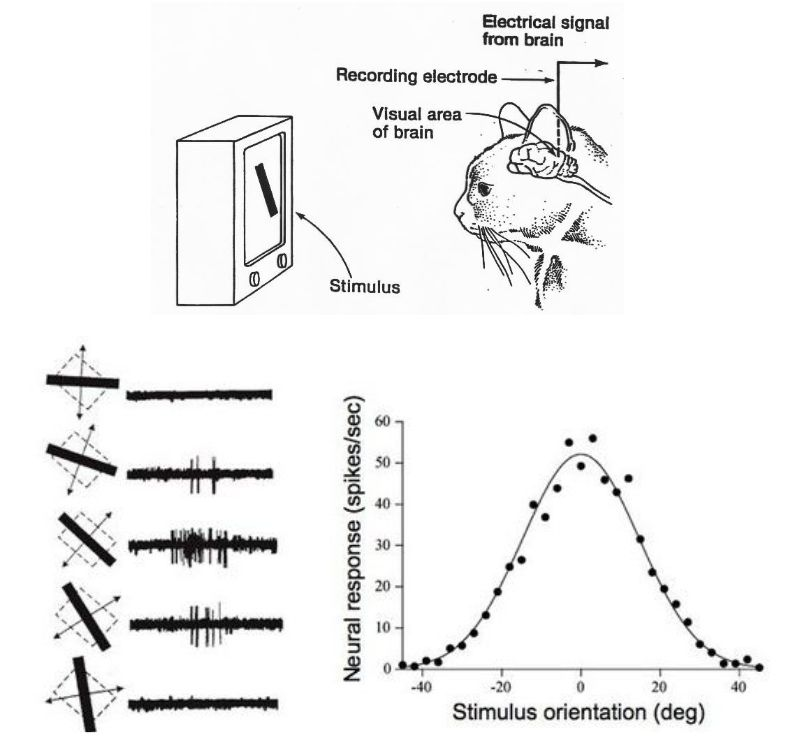
\includegraphics[keepaspectratio,
                                 width=\paperwidth,
                                 height=\paperheight]{cat_and_directions.jpeg}
            };
        \end{tikzpicture}
     \end{frame}
}


\begin{frame}
  \frametitle{Идея иерархической организации}
  \framesubtitle{История}
  \begin{center}
    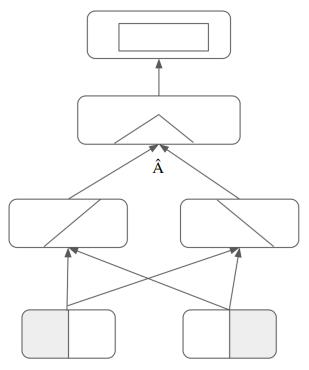
\includegraphics[keepaspectratio,
                     height=0.8\paperheight]{hierarchy_vision.jpg}
  \end{center}
\end{frame}


\begin{frame}
  \frametitle{Fukushima (1980)}
  \framesubtitle{История}
  \begin{center}
    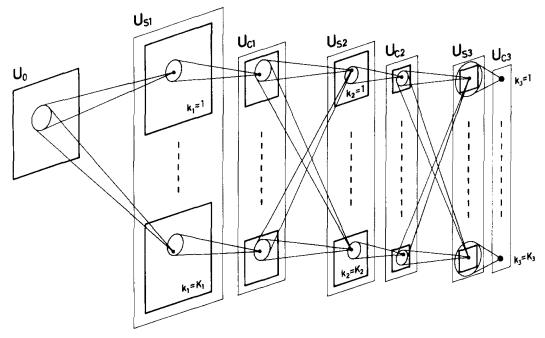
\includegraphics[keepaspectratio,
                     height=0.5\paperheight]{Fukushima_1980.png}
  \end{center}
  Уже использовались «свёртки» и активации, но без градиентного спуска и обучения с учителем
\end{frame}


\begin{frame}
  \frametitle{Lekun, Bottou, Bengio, Haffner (1998)}
  \framesubtitle{Первый успех}
  \begin{center}
    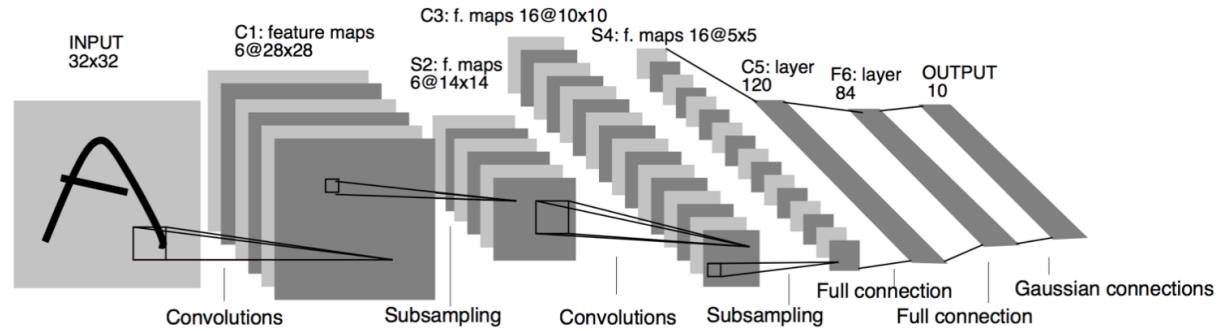
\includegraphics[keepaspectratio,
                     height=0.33\paperheight]{LeNet.jpg}
  \end{center}
\end{frame}


\begin{frame}
  \frametitle{Krizhevsky, Sutskever, Hinton (2012)}
  \framesubtitle{Настоящий прорыв}
  Победитель конкурса ImageNet того времени
  \begin{center}
    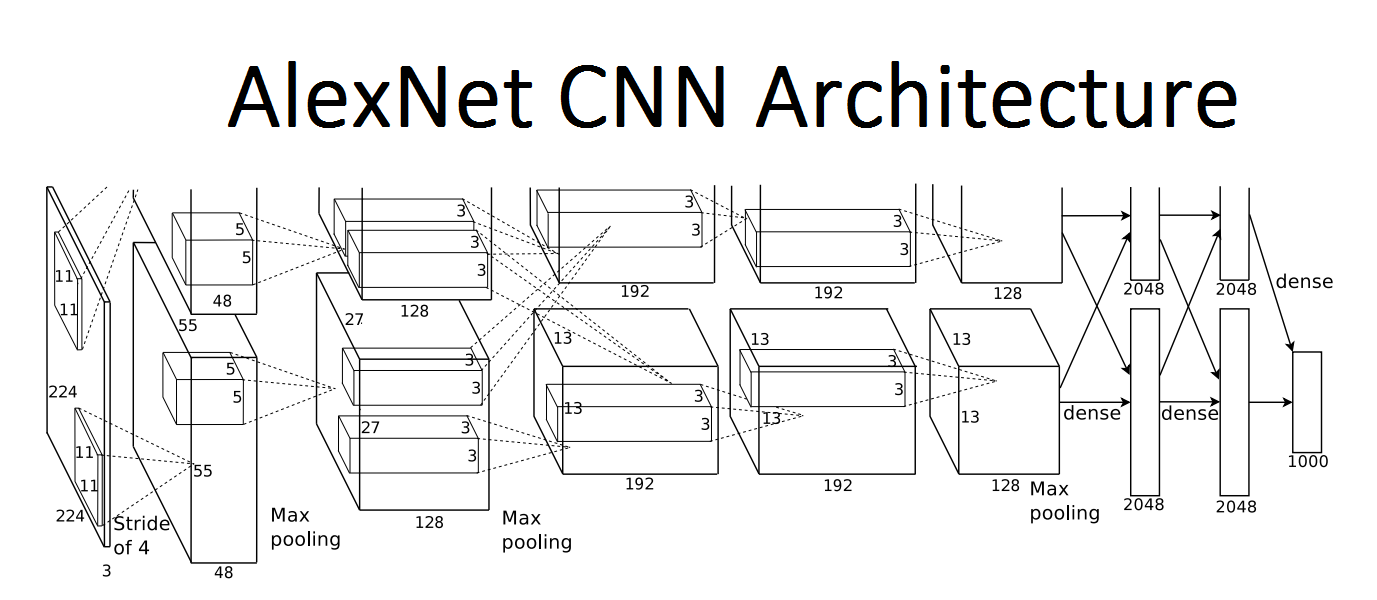
\includegraphics[keepaspectratio,
                     height=0.5\paperheight]{AlexNetCNN.png}
  \end{center}
\end{frame}


\begin{frame}
  \frametitle{Линейная модель}
  \framesubtitle{Напоминание}
  $f_j: X \to \mathbb{R}$ — числовые признаки

  $a(x, w) = \sigma(\left<w, x\right>) = \sigma \left(\sum\limits_{j=1}^n w_j f_j(x) - w_0 \right)$,

  где $w_0, w_1, \dots, w_n \in \mathbb{R}$ — веса признаков

  $\sigma(z)$ — функция активации, например, $\text{sign}(z),\ \frac{1}{1+e^{-z}},\ (z)_+$
  \begin{center}
    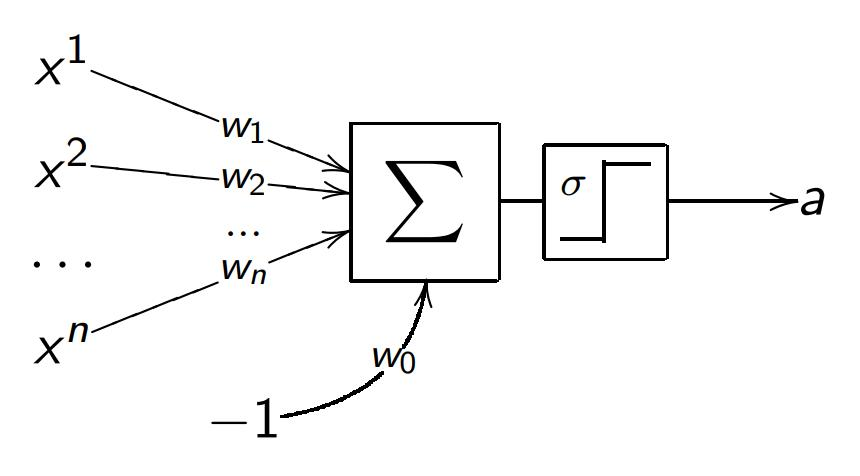
\includegraphics[keepaspectratio,
                     height=0.4\paperheight]{lin_as_nn.jpg}
  \end{center}
\end{frame}


\begin{frame}
  \frametitle{Нейронная сеть как комбинация линейных моделей}
  \begin{center}
    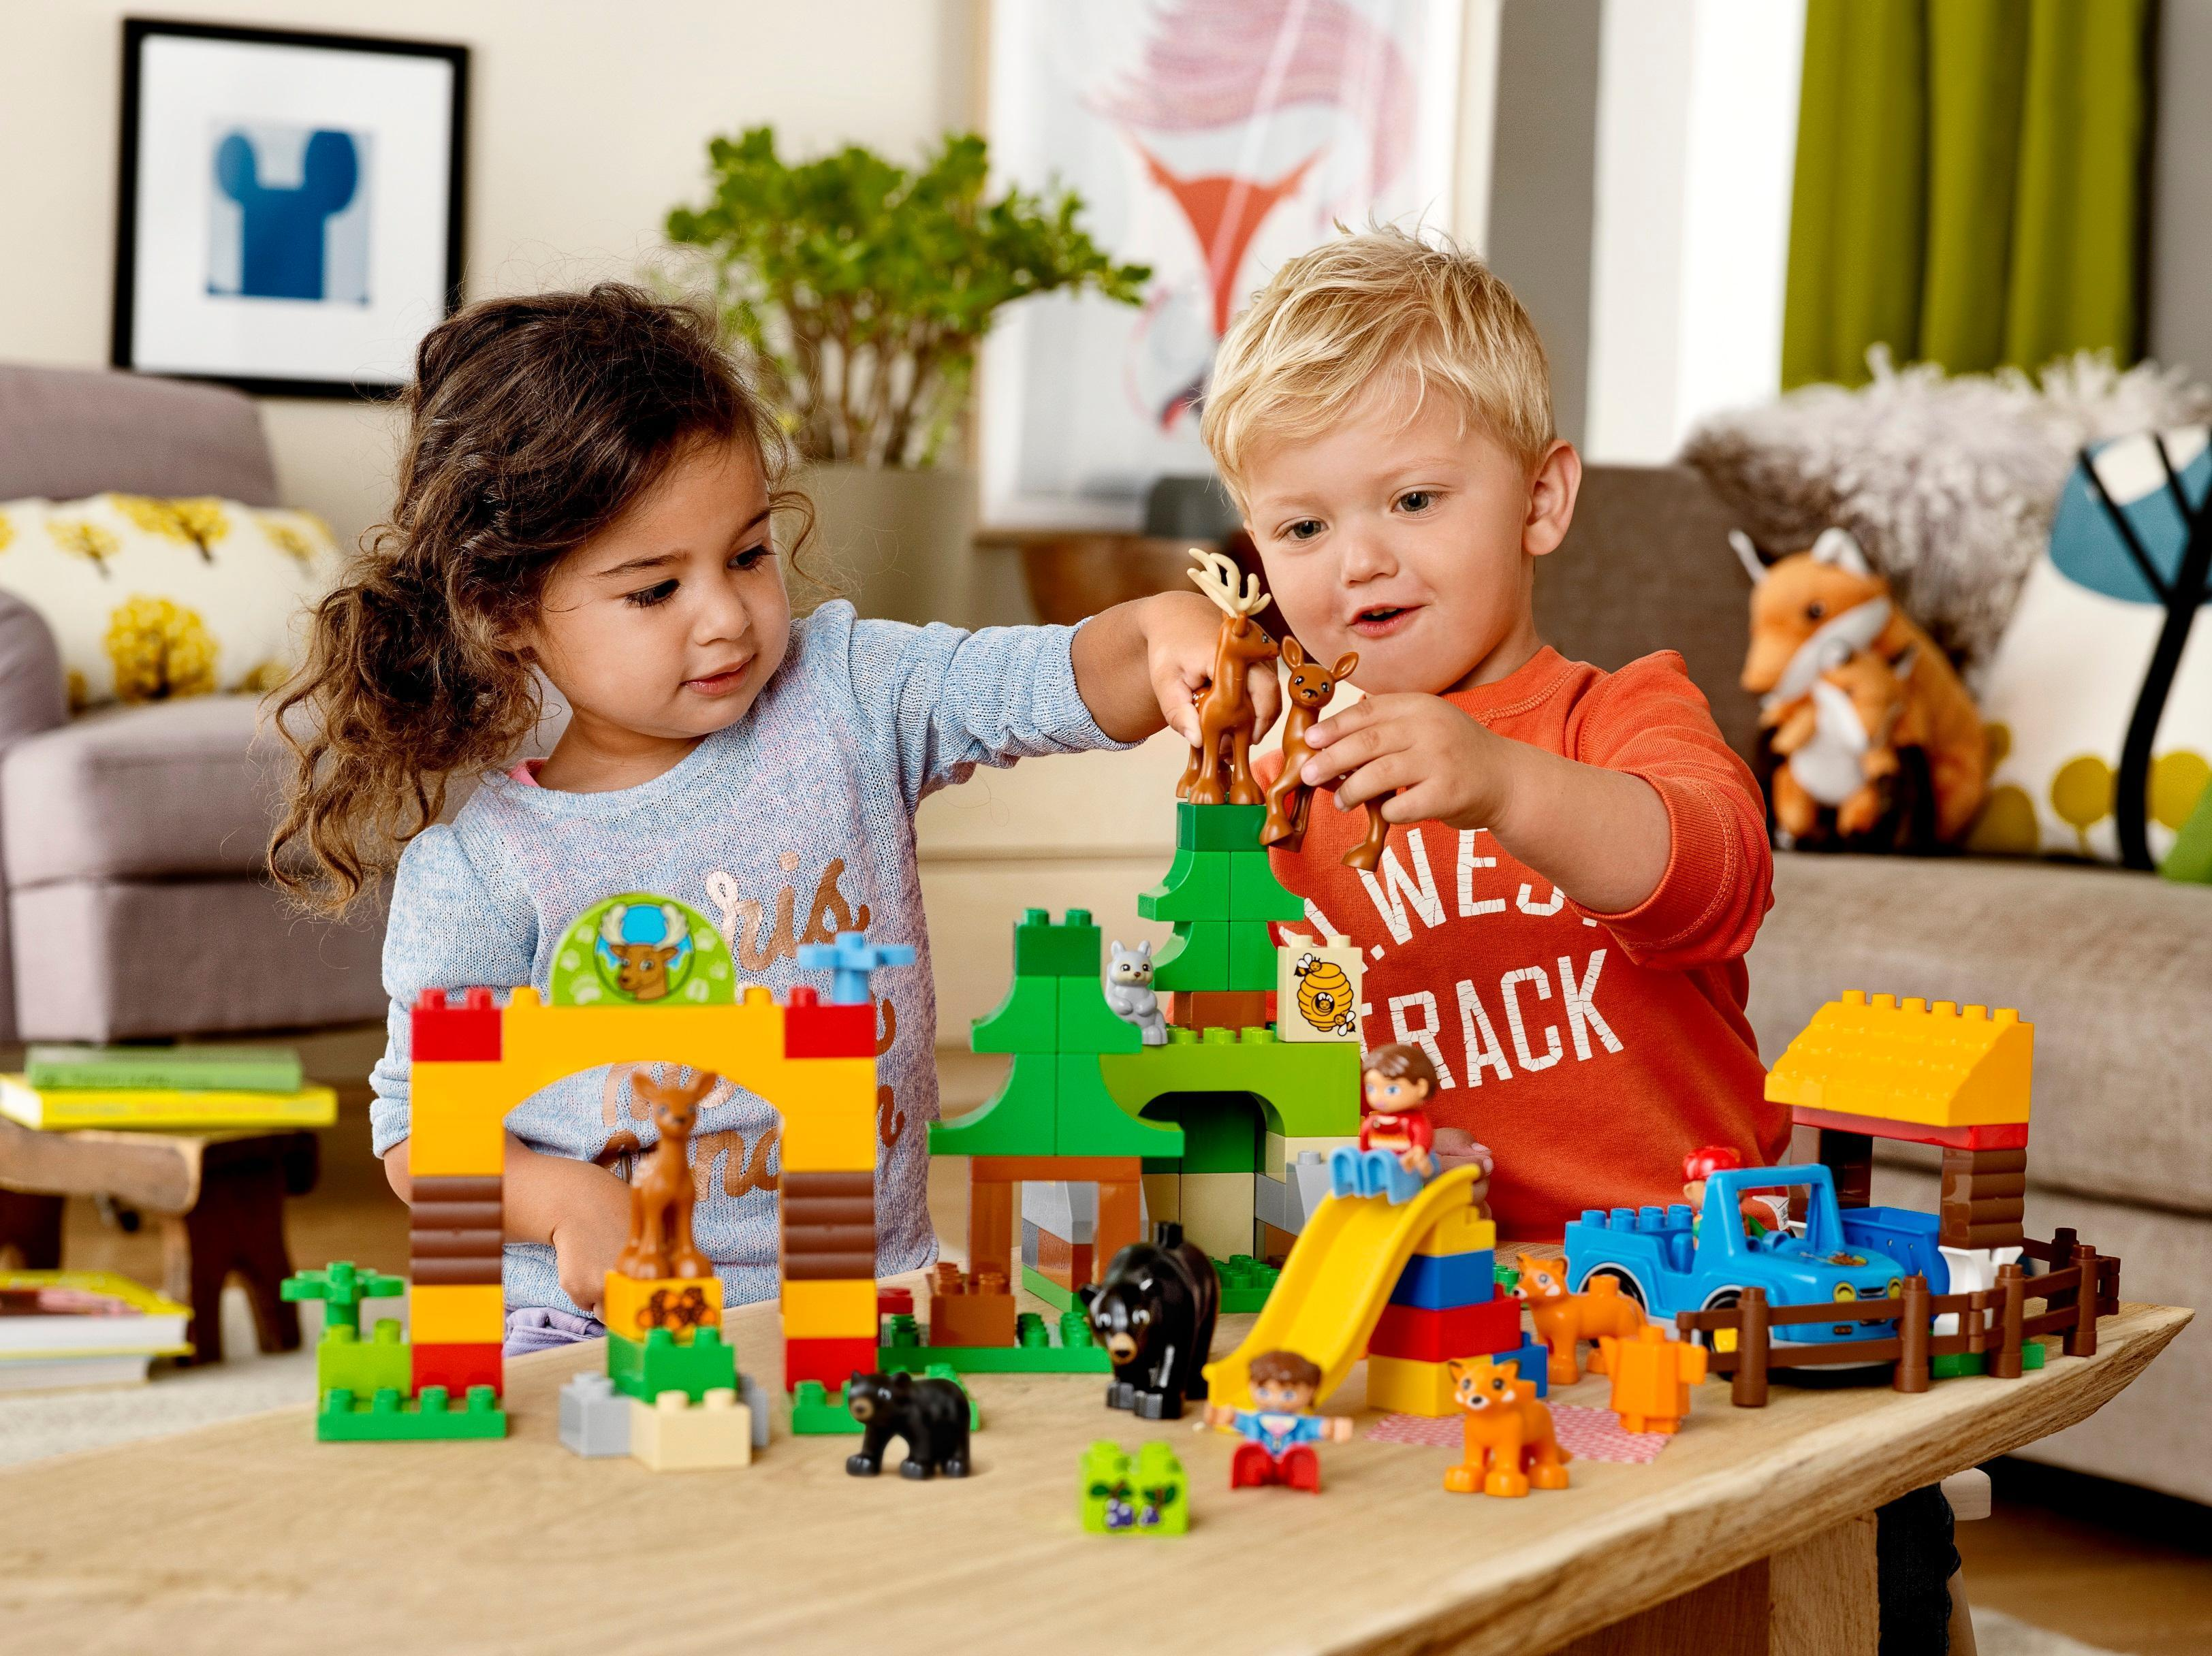
\includegraphics[keepaspectratio,
                     height=0.8\paperheight]{nn-as-lego-duplo.jpg}
  \end{center}
\end{frame}


\begin{frame}
  \frametitle{Свёрточная нейронная сеть}
  \begin{center}
    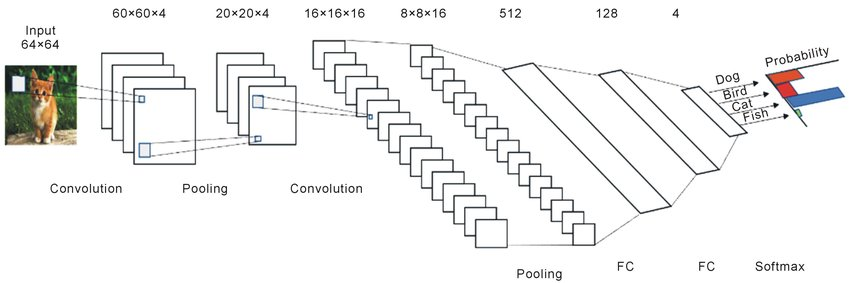
\includegraphics[keepaspectratio,
                     width=0.8\paperwidth]{cnn-example.png}
  \end{center}
\end{frame}


\begin{frame}
  \frametitle{Операция свёртки (convolution) в нейронных сетях}
  Свёртка в нейросетях — сумма произведений элементов
  \begin{center}
    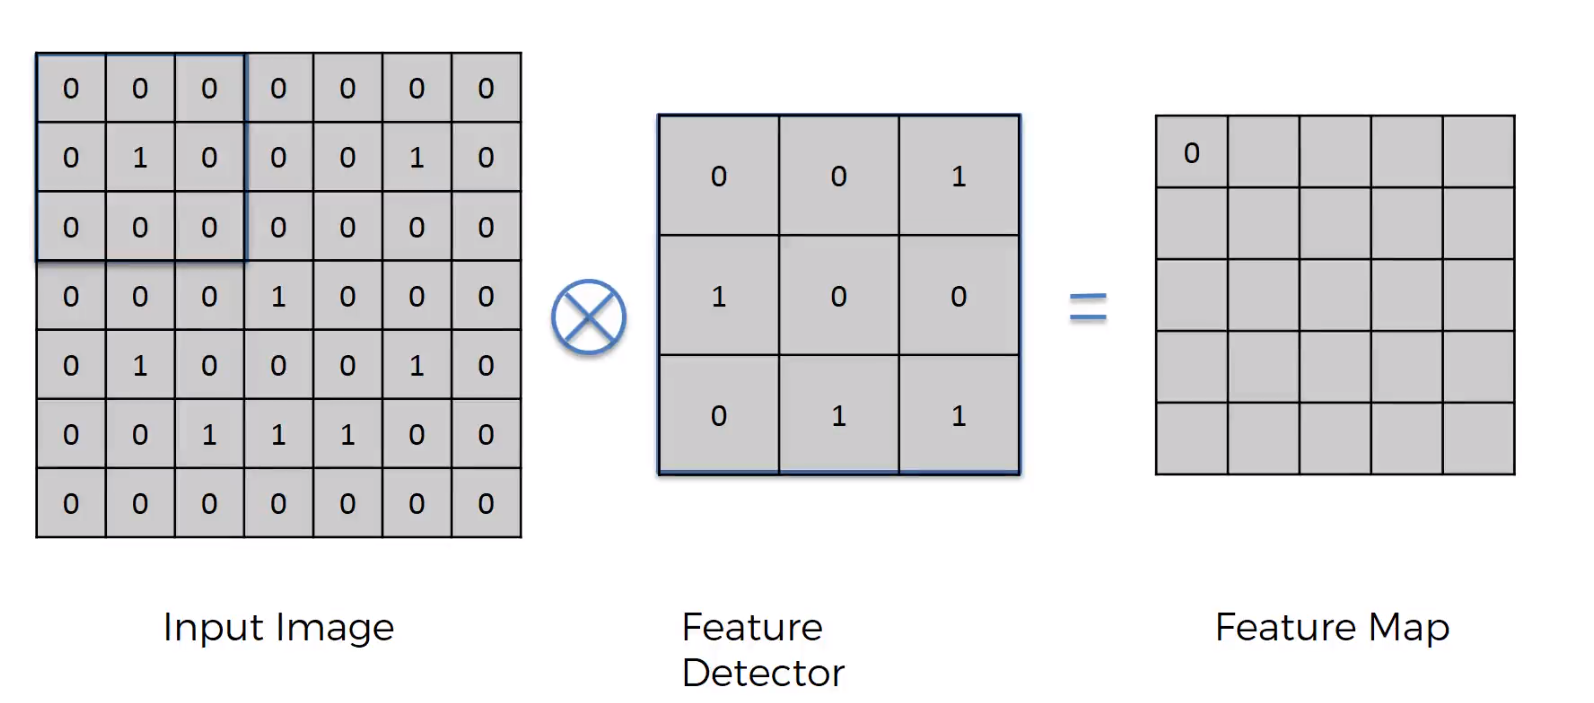
\includegraphics[keepaspectratio,
                     width=0.8\paperwidth]{conv-example.png}
  \end{center}
\end{frame}


\begin{frame}
    \begin{question}
    Почему «свёртка»?
    \end{question}
    \pause
    \begin{alertblock}{Замечание}
    При реализации свёртки эффективно умножается матрица на вектор. Вот, например, \href{https://arxiv.org/pdf/1509.09308.pdf}{статья с реализацией Winograd transformation} в cuDNN.
    \end{alertblock}
\end{frame}


\begin{frame}
  \frametitle{Пример операции свёртки}
  Ядро $3\times3\times3$ (Weight $\times$ Height $\times$ Channel numbers)
  \begin{center}
    \animategraphics[loop,width=0.7\paperwidth,autoplay]{1}{conv_live-}{0}{7}
  \end{center}
\end{frame}


\begin{frame}
  \frametitle{Дополнение (padding) и шаг (stride)}
  \begin{center}
    \animategraphics[loop,width=0.7\paperwidth,autoplay]{8}{padding_and_stride-}{0}{67}
  \end{center}
\end{frame}

\begin{frame}
  \frametitle{Расширение (dilation=2)}
  \begin{center}
    \animategraphics[loop,width=0.5\paperwidth,autoplay]{1}{dilation-}{0}{8}
  \end{center}
\end{frame}


\begin{frame}
  \frametitle{Считаем размер выхода}
  \begin{itemize}
    \item {\bf F}ilter size = 3x3 -> 3
    \item {\bf I}nput size = 5x5 -> 5
    \item {\bf S}tride = 1x1 -> 1
    \item {\bf P}adding = 0x0 -> 0
  \end{itemize}

  Output size = (I - F + 2*P)/S + 1 = (5 - 3 + 2*0)/1 + 1 = 3

  Output size = 3 -> 3x3
\end{frame}


\begin{frame}
  \frametitle{Пулинг (pooling, субдискретизация)}
  \begin{center}
    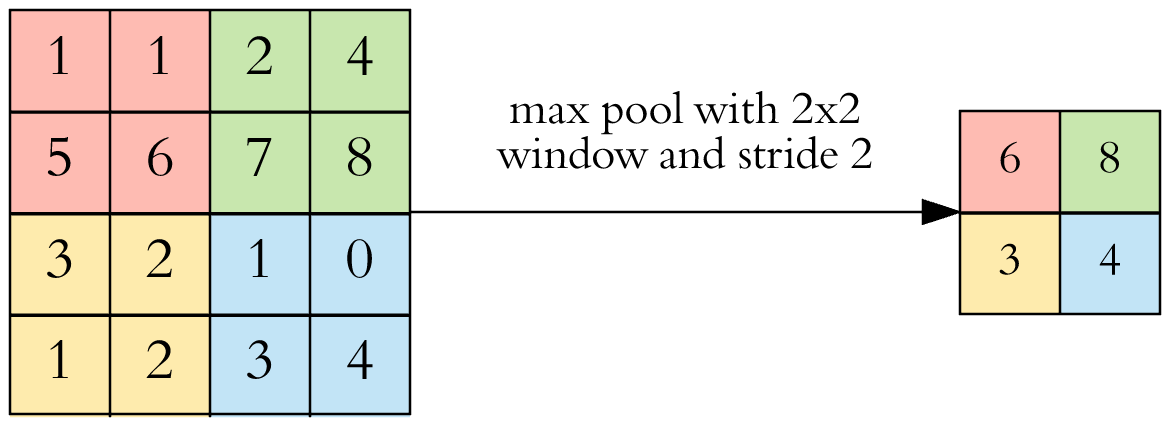
\includegraphics[keepaspectratio,
                     width=0.7\paperwidth]{max_pooling.png}
  \end{center}
\end{frame}


\begin{frame}
  \frametitle{Сигмоидальные функции активации}
  \framesubtitle{Функции активации}
  \begin{itemize}
    \item Логистический сигмоид
    $\sigma(z) = \frac{1}{1+\exp(-z)}$

    \item Гиперболический тангенс
    $\tanh(z) = \frac{\exp(z)-\exp(-z)}{\exp(z)+\exp(-z)}$

    \item непрерывные аппроксимации пороговых функций
    \item могут приводить к затуханию градиентов или «параличу» сети
  \end{itemize}
  \begin{question}
  Какие недостатки у логистического сигмоида?
  \end{question}
\end{frame}


\begin{frame}
  \frametitle{Посмотрим на графики}
  \begin{center}
    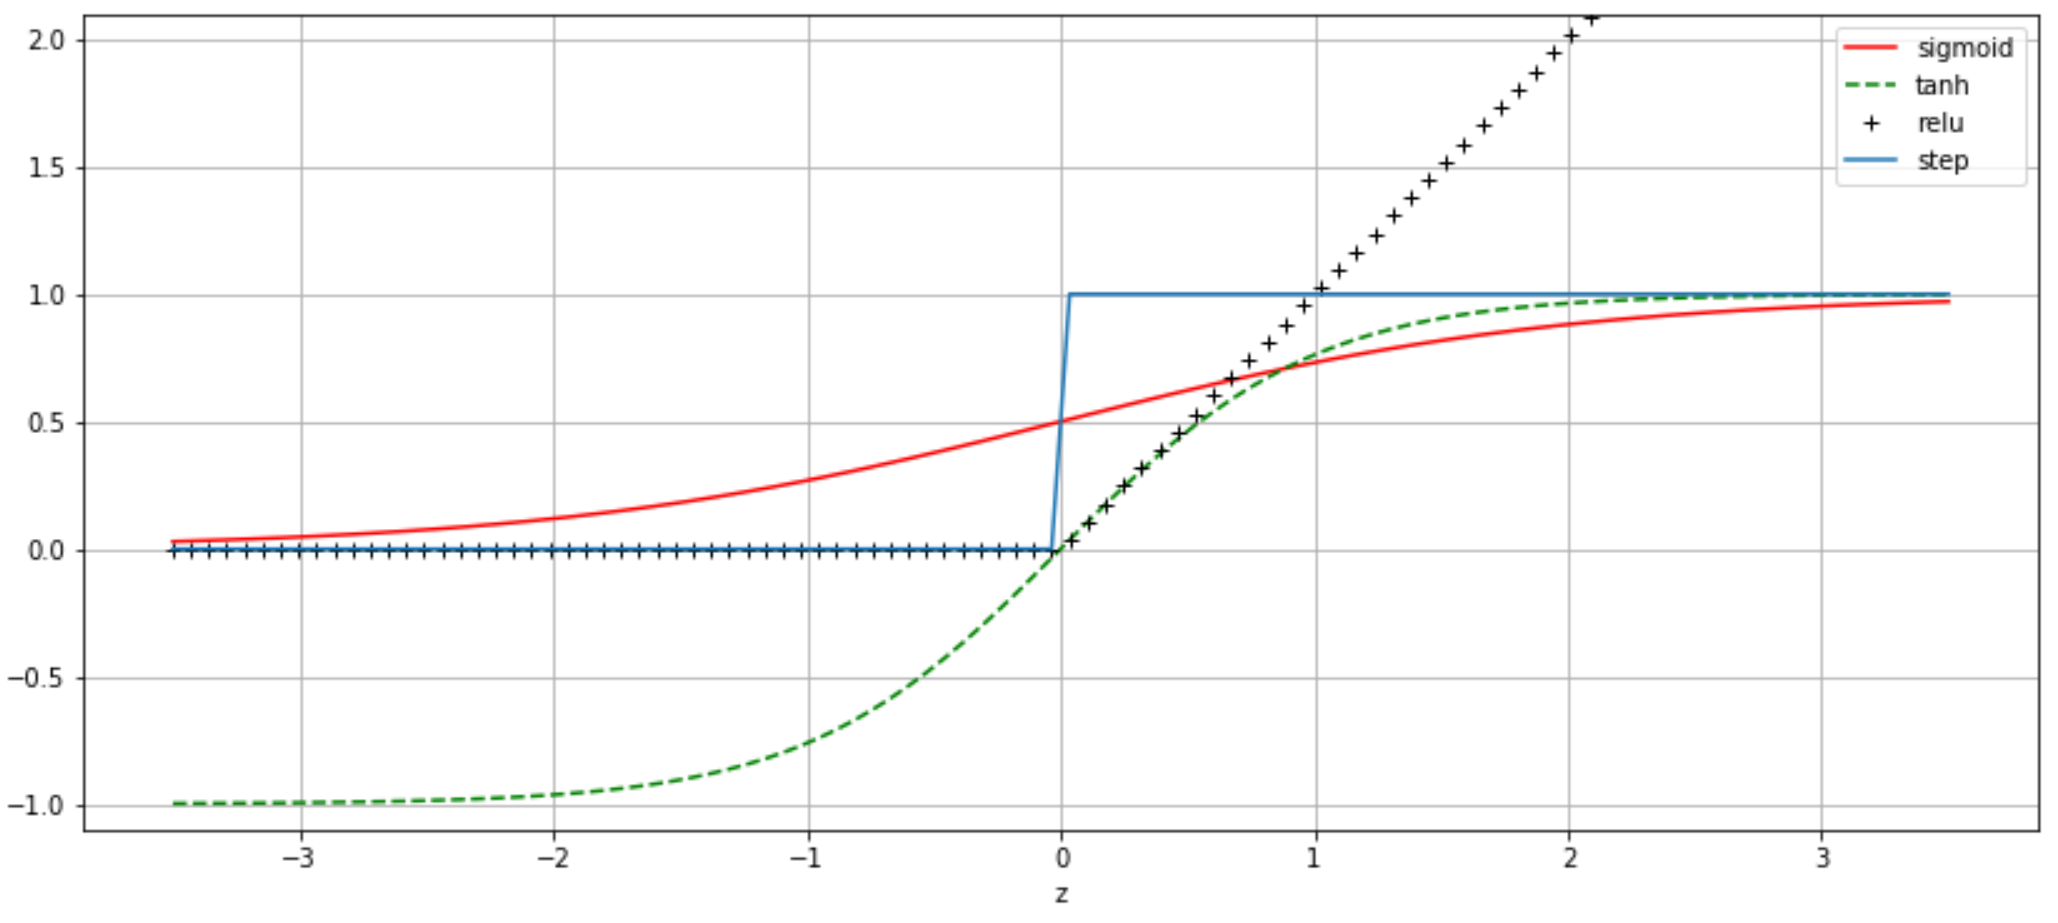
\includegraphics[keepaspectratio,
                     width=0.7\paperwidth]{sigm_relu.png}
  \end{center}
\end{frame}


\begin{frame}
  \frametitle{ReLU — Rectified Linear Unit}
  $$\text{ReLU}(z) = \max(0, z)$$

  Мотивация:

  $\sigma(5) \approx 0.9933, \sigma(10) \approx 0.9999$

  $f(x) = \sigma(x + \frac12) + \sigma(x - \frac12) + \sigma(x - \frac32) + \sigma(x - \frac52) + \dots$

  \begin{center}
    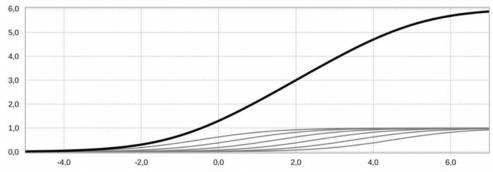
\includegraphics[keepaspectratio,
                     width=0.7\paperwidth]{from_nikolenko.jpg}
  \end{center}

  \noindent\rule{8cm}{0.4pt}

  Николенко С., Кадурин А., Архангельская Е. «Глубокое обучение», Питер, 2018. (стр. 107-113)
\end{frame}


\begin{frame}
  \frametitle{ReLU — Rectified Linear Unit}
  $$\int \sigma(x) dx = \log(1 + e^x) + C$$

  Получается, $f(x)$ — это риманова сумма вот такого интеграла:

  $$\int\limits_{1/2}^\infty \sigma(x + \frac12 - y) dy $$

  \begin{multline*}
    f(x) = \sum\limits_{i=0}^\infty \sigma(x + \frac12 - i) \approx \int \limits_{1/2}^\infty \sigma(x + \frac12 - y) dy = \\
    = [-\log(1 + \exp(x+\frac12 - y))]_{y=1/2}^{y=\infty} = \log(1 + \exp(x)) = \text{Softplus}(x)
  \end{multline*}
\end{frame}


\begin{frame}
  \frametitle{Посмотрим на графики}
  \begin{center}
    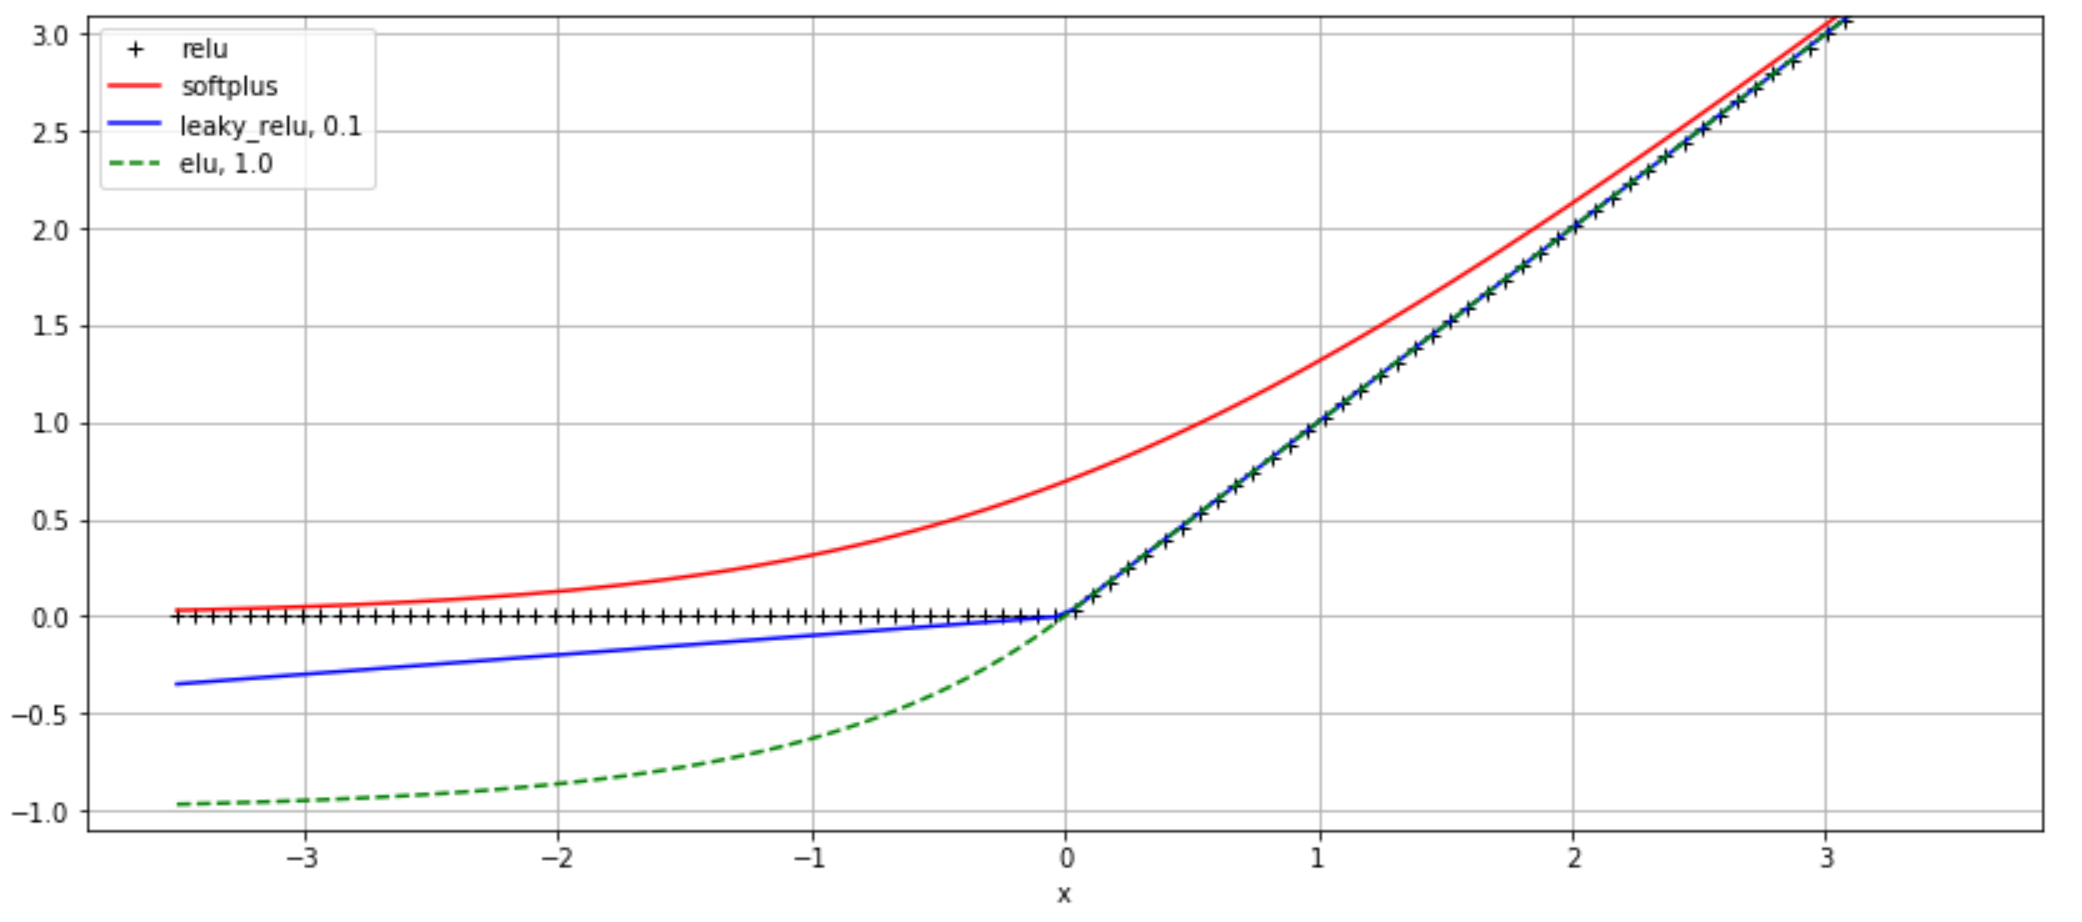
\includegraphics[keepaspectratio,
                     width=0.7\paperwidth]{relu_softplus.png}
  \end{center}
\end{frame}


\begin{frame}
  \frametitle{Развитие свёрточных сетей}
  \framesubtitle{или краткая история ImageNet}
  \begin{center}
    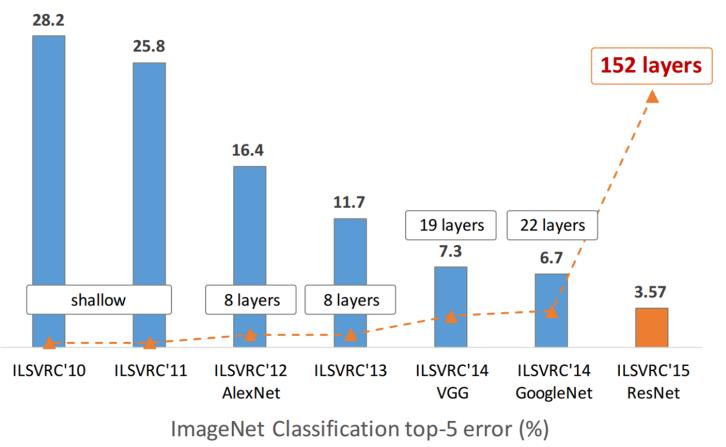
\includegraphics[keepaspectratio,
                     width=0.7\paperwidth]{image-net-history.jpg}
  \end{center}
\end{frame}


\begin{frame}
  \begin{question}
  Что такое ImageNet?
  \end{question}
\end{frame}


\begin{frame}
  \frametitle{ImageNet}
  Проект массивной базы данных аннотированных изображений:
  \begin{itemize}
    \item 14M+ изображений
    \item 20K+ классов
  \end{itemize}

  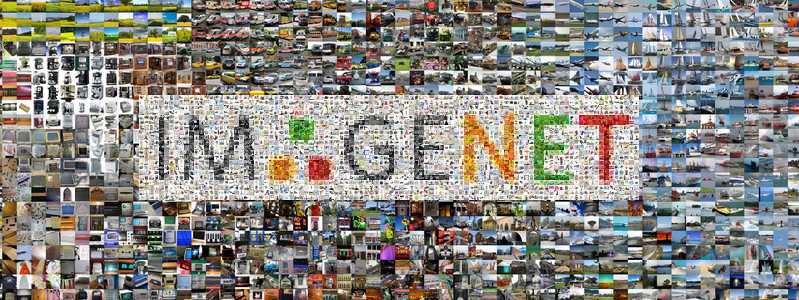
\includegraphics[keepaspectratio,
                   width=0.85\paperwidth]{ImageNet-Large-Scale.jpg}
\end{frame}


\begin{frame}
  \frametitle{AlexNet (Krizhevsky, Sutskever, Hinton, 2012)}
  \framesubtitle{Победитель конкурса ImageNet того времени}
  \begin{center}
    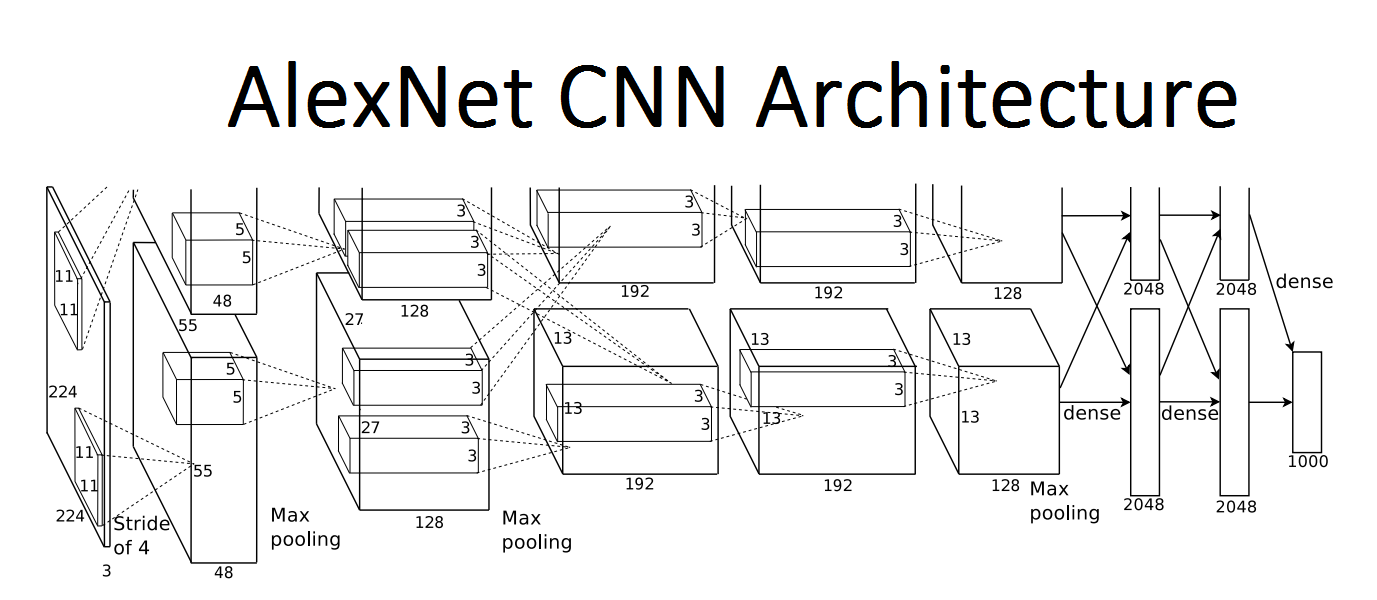
\includegraphics[keepaspectratio,
                     width=0.5\paperwidth]{AlexNetCNN.png}
  \end{center}
  \begin{itemize}
    \item ReLU
    \item аугментация данных
    \item {\it dropout 0.5}
    \item {\it batch normalization} (размер батча 128)
    \item SGD Momentum 0.9
    \item L2 регуляризация 5e-4
    \item Learning rate 1e-2, потом уменьшение в 10 раз после стабилизации качества на тесте
  \end{itemize}

    Финальное качество top5 на ImageNet — 25.8\% ->16.4\%
\end{frame}


\begin{frame}
  \frametitle{Метод накопления импульса (momentum method)}
  Метод накопления импульса [Б.Т.Поляк, 1964] — экспоненциальное скользящее среднее градиента по $\frac{1}{1-\gamma}$ последним итерациям:

  \begin{tabular}{lr}
    $\nu = \color{red}{\gamma} \nu + \color{red}{(1-\gamma)} \mathcal{L}_i^\prime(w)$ &
    \multirow{2}{*}{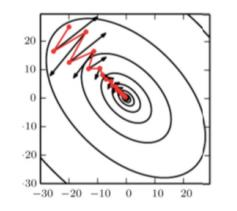
\includegraphics[keepaspectratio,
                     width=0.3\paperwidth]{momentum_2.jpg}} \\
      $w = w - \eta \nu$ &
  \end{tabular}

\end{frame}


\begin{frame}
  \frametitle{Поправка Нестерова (1983)}

\begin{tabular}{lr}
  $\nu = \gamma \nu + (1 - \gamma) \mathcal{L}_i^\prime (w \color{red}{- \eta \gamma v})$ &
  \multirow{2}{*}{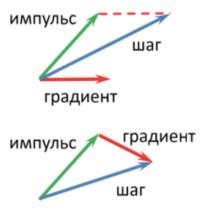
\includegraphics[keepaspectratio,
                   width=0.3\paperwidth]{nesterov.jpg}} \\
    $w = w - \eta \nu$ &
\end{tabular}

\end{frame}


\begin{frame}
  \frametitle{Резюме}
  \begin{itemize}
    \item Свёрточные сети очень хорошо подходят для обработки изображений
    \item По-видимому немного похожи на механизмы биологического зрения
    \item При этом гибкие и вычислительно эффективные
    \item Сегодня фактический стандарт для задач компьютерного зрения (классификация, детекция, сегментация, генерация)
    \pause
    \item Будет на следующей лекции
      \begin{itemize}
        \item различные алгоритмы оптимизации: adam, RMSProp
        \item dropout
        \item выбор начального приближения
        \item ResNet и WideResNet
      \end{itemize}
  \end{itemize}

  \pause
  Что ещё можно посмотреть?
  \begin{itemize}
    \item \href{https://cs.stanford.edu/people/karpathy/convnetjs/}{Демо от Андрея Карпаты}
    \item Есть курс Стенфорда «CS231n: сверточные нейронные сети для визуального распознавания»: http://cs231n.github.io/
  \end{itemize}
\end{frame}

\end{document}
